\documentclass{scrartcl}
\usepackage[utf8]{inputenc}
\usepackage{hyperref}
\usepackage{url}
\usepackage{natbib}
\usepackage{graphicx}
\usepackage{cleveref} % this must be the last package to be loaded

\newcommand{\emailaddr}[1]{\href{mailto:#1}{\texttt{#1}}}

\title{\LARGE
    Final Report Template\\
    DS-Monopoly
}
\subtitle{Final Report for the Distributed Systems Course [2025/2026]}

% Consider watching:
% https://www.youtube.com/watch?v=ihxSUsJB_14
% https://www.youtube.com/watch?v=XTFWaV55uDo

\author{
    Daniele Loverre \\ \emailaddr{daniele.loverre@studio.unibo.it}
}

\date{\today}

\begin{document}
\nocite{*}

\maketitle

\begin{abstract}
  DS-Monopoly is a distributed clone of the Monopoly board game.
    It is a simplified version of the game where a centralized server acts as the \textit{bank},
  it coordinates the game and keeps the game state, validates actions, prevents cheating and
  broadcasts the updates to all the connected clients.
  The clients are \textit{players} that can join a game by connecting to the central server (2 to 4 players per game).
  Players can buy properties or houses, roll dice and see the board and the players information from a GUI.
  Disconnections from both sides, clients and server, are handled in order to keep the game running.
  Features like checkpointing, authentication and timeouts, are used to enhance fault tolerance and
  ensure more reliability and availability.
\end{abstract}

\section*{Disclaimer}

During the preparation of this work, the author used Gemini to assist in coding the graphical user interface
with PyGame for the clients, the unit tests and to accelerate the development of some small functions and code refactoring.
It was not used to design the project's architecture.

After using this tool/service, 
the author reviewed and edited the content as needed
and takes full responsibility for the content of the final report/artifact.

\section{Concept}\label{concept}

The project is a desktop application with a GUI for clients.
Players can see the board with houses built and pawns on it on the left,
and the information of the players, such as their balance and their properties, on the right.
The last event of the game is also written on the GUI in order to
let players understand what happens during their and others player's turn.
The server can be started on CLI or using docker compose, all the information and logs of the server can be read on CLI.


Players cannot play on the same device (more precisely on the same window).
They connect to a server, providing the server's port and ip,
provided on the server's CLI at the start, and an available nickname.
Clients send messages every event they generate, created on button's pressing.
The server broadcasts to all his connected clients the game state on every update on it.
They exchange messages in JSON sent via TCP socket.
The only data stored are the checkpoint of the game state saved in a file on the server side
and the tokens saved in files for the authentication, one for each nickname used, on the client side.


When the server is started the game waits for clients to connect.
Once all the players in the \textit{lobby} are ready (at least 2 players)
the game starts, 5000 coins and 5 random properties are assigned to each player.
Following their turn, players can make actions that are sent to the server and updates the game state.
The updated state is sent back to all the players.
The game continues until only one players remains without going in \textit{bankruptcy}
or until all the players left the game.


Distribution is needed in this project to allow geographical distribution between nodes,
so that is not necessary that players are in the same physical room, but the game state is shared across the network.
The state is kept only on the server that acts as a single source of truth, avoiding cheating from clients.
Furthermore, the failure of a client does not interrupt the game, but it can be continued by the other players connected.

\section{Requirements Elicitation and Analysis}\label{requirements}
\subsection{Functional requirements}\label{functional_requirements}

\begin{itemize}
    \item \textbf{Server Initialization:} The server should expose and print its endpoint (IP and port) upon startup.
    \begin{itemize}
        \item \textit{Acceptance Criterion:} Running the server application outputs its endpoint on the CLI.
    \end{itemize}

    \item \textbf{Client Connection:} Clients should be able to connect to the server using the provided endpoint and an available nickname, opening a GUI lobby.
    \begin{itemize}
        \item \textit{Acceptance Criterion:} A user entering a valid IP, port, and unique nickname successfully joins the lobby and sees the GUI.
    \end{itemize}

    \item \textbf{Game Start Condition:} The game should start only when at least two players are in the lobby and all connected players pressed \textit{"ready"}.
    \begin{itemize}
        \item \textit{Acceptance Criterion:} The game goes from lobby to playing state immediately after the last player clicks the ready button.
    \end{itemize}

    \item \textbf{Turn Management:} The system should have a turn-based logic, each player can only do the actions they are allowed to do during their specific turn.
    \begin{itemize}
        \item \textit{Acceptance Criterion:} A player cannot click \textit{"roll dice"} or \textit{"buy"} if it is not their turn or if the action is invalid for their current state.
    \end{itemize}

    \item \textbf{Game State Visualization:} The GUI should display the game board, player information (balance, properties), and the last game event.
    \begin{itemize}
        \item \textit{Acceptance Criterion:} Whenever an action is performed, the GUI immediately updates the board, the balances, and the event log for all connected players.
    \end{itemize}

    \item \textbf{Client Disconnection Handling:} If a client disconnects, the game should pause and grant the disconnected player 30 seconds to rejoin.
    \begin{itemize}
        \item \textit{Acceptance Criterion:} A disconnection triggers a 30-second timer; if the player reconnects in time, the game resume. Otherwise, the player goes bankrupt.
    \end{itemize}

    \item \textbf{Server Disconnection Handling:} If the server fails, clients should wait up to 90 seconds for it to restart before shutting down.
    \begin{itemize}
        \item \textit{Acceptance Criterion:} Shutting down the server triggers a 90-second waiting state on all active clients.
    \end{itemize}

    \item \textbf{Winning Condition:} The game should end when only one player remains active and not in bankruptcy.
    \begin{itemize}
        \item \textit{Acceptance Criterion:} When all the players, except one, declare bankruptcy or disconnect permanently, the system declares the remaining player the winner.
    \end{itemize}
\end{itemize}

\subsection{Non-functional requirements}\label{non_functional_requirements}

\begin{itemize}
    \item \textbf{Consistency:} The system should ensure state consistency across all connected nodes at any given time.
    \begin{itemize}
        \item \textit{Acceptance Criterion:} The players GUI's will always show the exact same data.
    \end{itemize}
    \item \textbf{Security:} The system should prevent clients from doing invalid game actions.
    \begin{itemize}
        \item \textit{Acceptance Criterion:} Any altered or malicious payload sent by a client is rejected by the server without affecting the game state.
    \end{itemize}
    \item \textbf{Availability and Fault Tolerance:} The system should be able to recover its exact previous state following a critical node failure.
    \begin{itemize}
        \item \textit{Acceptance Criterion:} Restarting the server after a simulated crash allows clients to reconnect and find the board, balances, and turn order exactly as they were before the crash.
    \end{itemize}
\end{itemize}

\subsection{Implementation requirements}\label{implementation_requirements}

\begin{itemize}
    \item \textbf{Programming Language:} The system is developed using Python.
    \item \textbf{Networking Protocol:} The communication between client and server is
                                              implemented using TCP sockets to ensure reliable delivery.
    \item \textbf{Data Format:} Nodes exchange information using the JSON format.
    \item \textbf{GUI Library:} The client's graphical interface is built using the PyGame library.
    \item \textbf{Containerization:} The server can be started using Docker Compose to facilitate
                                            automatic restarts and environment consistency.
\end{itemize}

\subsection{Relevant Distributed System Features}
\label{ds-features}

\begin{itemize}
  \item \textbf{Transparency:}
  The clients only need a single network endpoint (IP and port) to interact with the service,
  the internal server hosting details are hidden.
  However, full transparency (such as failure or replication transparency) is not a primary goal;
  failures and reconnection states are explicitly made visible to the players via the GUI to manage expectations during network drops.

  \item \textbf{Fault Tolerance and Dependability:}
  If a client fails, recovery systems try to reestablish all the connection and resume the game.
  The server needs to be active for the entire game, but, if a failure occurs,
  it should be able to reload the game state from the last saved checkpoint.
  The checkpoint must be available and not corrupted in order to be used in a server reconnection.
  The reconnections timeouts are 30 seconds for the clients and 90 seconds for the server.
  When a client fails, the reconnection timeout should restart also for the other disconnected players.

  \item \textbf{Scalability:}
  At the moment a server can handle one single game concurrently.
  The system could need to handle an increasing number of users when more lobbies can be created on a single server.
  The amount of data handled should be more or less the same even if the complexity of the game increases as the actual real game is.
  Each game is independent, so at the end of the game everything is reset.


  \item \textbf{Security and Trust:}
  The only data stored are the checkpoint on server's side and the token file for authentication on client's side.
  Cheating is prevented by having a centralized server, clients can only read the serialized game state and cannot communicate to other clients.
  Every player has the same permission.
  The authentication is needed for guarantee that a player that reconnects to a game after
  a failure is the exact same player that was playing before the failure occurred.

  \item \textbf{Resource Sharing:}
  The \textit{game state} is the resource kept by the central server.
  The server coordinates and synchronize the process, it handles the incoming events from clients,
  updates the game state and broadcasts it to the connected peers.
  The clients cannot access the \textit{game state} directly, they cannot read it or modify it directly,
  but they can only generate events that the server elaborates in order to modify and send the \textit{game state}.

  \item \textbf{Communication Efficiency and Bandwidth:}
  The game is turn-based, there is no need to have an instant update from the server.
  All the data sent on the network has almost the same size, from the server is the game state and from the clients the events they generate.
\end{itemize}

\section{Design}\label{design}

This chapter explains the strategies used to meet the requirements identified in the analysis.

\subsection{Architecture}\label{architecture}
The system adopts a \textbf{Client-Server} architecture.
The central server acts as the manager of the game logic and the single source of truth for the shared game state.
On the other hand the clients responsibilities are rendering the Graphical User Interface (GUI),
capturing player inputs, and forwarding the events to the server.


This choice was made to ensure different requirements and features identified in Section\ref{requirements} and Section\ref{ds-features}:
\begin{itemize}
    \item \textbf{Security and Anti-Cheating:} By establishing an authoritative server, clients cannot manipulate the game.
    The server strictly validates every requested action against the game rules before applying it and broadcasting the result.
    \item \textbf{Consistency:} In a turn-based board game, all players must observe the exact same state simultaneously.
    A centralized server resolves concurrency issues, processing incoming events sequentially and ensuring that no state divergence occurs among the connected nodes.
    \item \textbf{Network and Algorithmic Simplicity:} A P2P architecture would have required a fully connected mesh network and
    complex distributed consensus algorithms just to agree on simple game events like dice roll or a property purchase.
    The Client-Server model drastically reduces network overhead and algorithmic complexity.
\end{itemize}

\subsection{Infrastructure}\label{infrastructure}

The system architecture follows a classic Client-Server model.
The infrastructure is designed to be lightweight, avoiding external dependencies such as dedicated databases, message brokers, or load balancers.

\subsubsection{Infrastructural Components}
The system has the following infrastructural components:
\begin{itemize}
    \item \textbf{Central Server (1 instance):} It acts as the game coordinator and the single source of truth.
        It manages connections, holds the authoritative game state in-memory, validates actions, and broadcasts updates to the connected peers.
    \item \textbf{Game Clients (2 to 4 instances):} These represent the end-users.
        They are responsible for rendering the graphical user interface (GUI) and forwarding user inputs to the server.
        Clients do not communicate with each other directly, all traffic passes through the server.
    \item \textbf{Storage (Local File System):} Instead of a traditional database, the server uses the host's local file system
        to store checkpoints (\texttt{autosave.json}) and the clients use it to store authentication tokens.
        This ensures fault tolerance and session recovery without the overhead of maintaining a database server.
\end{itemize}

\subsubsection{Network Distribution}
The components are designed to be distributed over the network.
The server and clients typically run on different machines.
The server binds to the machine's local IP, and clients connect over the network using standard TCP sockets.

\subsubsection{Component Discovery}
The system relies on explicit endpoint provisioning:
\begin{enumerate}
    \item Upon startup, the Server inspects its network interfaces and logs its binding endpoints (IP addresses and port) to the terminal.
    \item The end-users explicitly provide the target IP and port to their Client application upon launch.
    \item Once connected, the server assigns a unique authentication token to the client, guaranteeing safe reconnection to the session even if the IP changes dynamically.
\end{enumerate}

\vspace{0.5cm}
\begin{figure}[h]
    \centering
    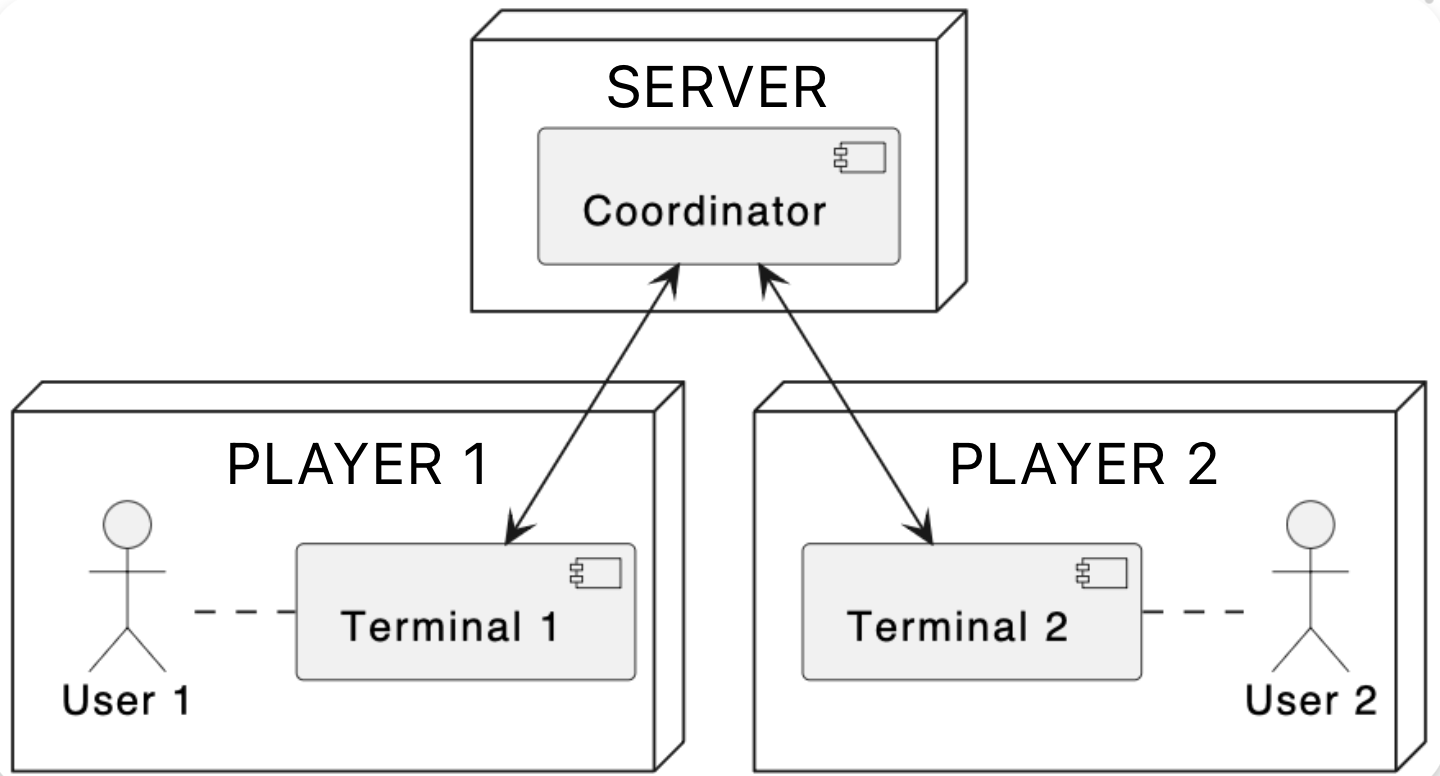
\includegraphics[width=0.8\textwidth]{figures/components}
    \caption{Component diagram of the Monopoly system with two players.}
    \label{fig:infrastructure}
\end{figure}
\vspace{0.5cm}

\subsection{Modelling}\label{modelling}

\subsubsection*{Domain Entities}
The primary domain entities are:
\begin{itemize}
    \item \textbf{\texttt{Monopoly}:} The root entity representing the game session, managing the lifecycle (lobby, playing, paused, closed), turns, and the list of players.
    \item \textbf{\texttt{Player}:} Represents a user in the game. It holds personal state such as balance, board position, owned properties, and bankruptcy status.
    \item \textbf{\textbf{\texttt{Board}} \& \textbf{\texttt{Space}}:} The physical representation of the game. The Board is an aggregate of multiple Spaces, which are divided into \texttt{PropertySpace} (can be bought, owned, and upgraded with houses) and \texttt{ActionSpace} (trigger special events like Taxes, Jail, or Chance cards).
\end{itemize}

\subsubsection*{Mapping to Infrastructural Components}
\begin{itemize}
    \item The true, mutable \textbf{state of the domain entities} resides entirely in the memory of the central server (\texttt{MonopolyBank}).
    \item The server periodically save the state to the local file system via the Checkpointing module.
    \item The clients (\texttt{MonopolyUser}) only receive a serialized representation (a JSON dictionary) of the state. Clients render the representation visually and collect user inputs.
\end{itemize}

\subsubsection*{Domain Events}
In this architecture the domain events are modeled by the \texttt{PlayerEvent} enumeration:
\begin{itemize}
    \item \textbf{Lifecycle Events:} \texttt{JOIN}, \texttt{READY}, \texttt{DISCONNECTION}, \texttt{RECONNECTION\_TIMEOUT}, \texttt{QUIT}.
    \item \textbf{Gameplay Events:} \texttt{ROLL} (moves the player and evaluates the landing space), \texttt{BUY} (purchases a property), \texttt{BUILD} (adds a house), \texttt{END\_TURN} (shifts the turn to the next player).
\end{itemize}

\subsubsection*{Exchanged Messages}
Communication between components relies on asynchronous JSON messages over TCP, categorized into:
\begin{itemize}
    \item \textbf{Events (Client $\rightarrow$ Server):} Sent by the user. They contain the event type and a payload (e.g., \texttt{\{"type": "roll", "payload": \{"nickname": "Alice"\}\}}).
    \item \textbf{State Updates (Server $\rightarrow$ Client):} The server responds to valid commands by broadcasting the entire updated, serialized game state to all connected peers.
\end{itemize}

\subsubsection*{System State Comprehension}
The global state of the system encapsulates all the information required to resume or render the game at any exact moment. It comprehends:
\begin{itemize}
    \item \textbf{Game Data:} Current status (LOBBY, PLAYING, PAUSED, CLOSED), active turn index, \texttt{has\_rolled} flags, and a list of allowed actions for the current UI generation.
    \item \textbf{Players' Data:} Nicknames, board positions, balances, and boolean flags for bankruptcy.
    \item \textbf{Board Data:} The structural layout of the spaces, including dynamic data like the \texttt{owner} of each property and the number of \texttt{houses} built on them.
    \item \textbf{Network State:} Sets of ready players and sets of temporarily disconnected players waiting for reconnection.
\end{itemize}

\vspace{0.5cm}
\begin{figure}[h]
    \centering
    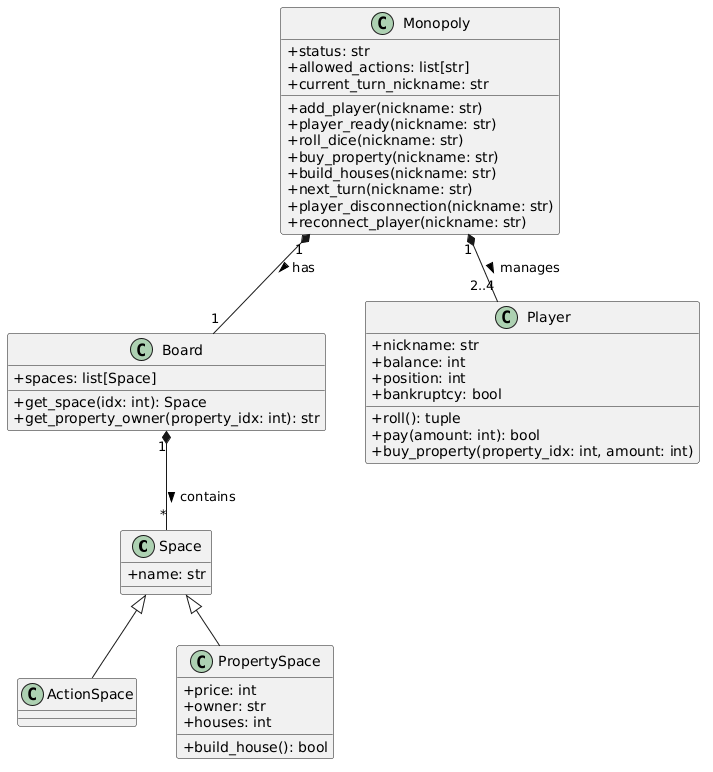
\includegraphics[width=0.8\textwidth]{figures/model_diagram}
    \caption{Class diagram of the model's main components.}
    \label{fig:model class diagram}
\end{figure}
\vspace{0.5cm}

\subsection{Interaction}\label{interaction}

The communication between components is asynchronous and relies on exchanging serialized JSON strings over TCP sockets.
The interaction architecture avoids peer-to-peer communication: all clients communicate exclusively with the central server.

\subsubsection*{Interaction Patterns}
The clients never calculate game logic (e.g., they do not compute dice rolls or property costs).
They strictly send user events and wait.
The Server is the sole authority that executes the logic and determines the outcome.
Instead of clients polling the server for updates, the server proactively broadcasts the entire serialized game state to all connected peers every time a mutation occurs.
Upon receiving a new state, the client's GUI inspects the \texttt{current\_turn\_nickname} and \texttt{allowed\_actions} fields to dynamically determine whether to enable the input buttons for the local user.


\subsubsection*{Communication Flow}
Communication is triggered purely by user inputs (e.g., clicking a button) or connection lifecycle events (e.g., socket closed).
Clients send lightweight JSON payloads containing an action type (e.g., \texttt{join}, \texttt{ready}, \texttt{roll}) and a payload specifying the actor's nickname and token.
The server responds by broadcasting the full, heavy JSON representation of the entire Monopoly object, ensuring all clients are perfectly synchronized.


\subsubsection*{Sequence Diagram}
Figure~\ref{fig:sequence_diagram} illustrates the initialization phase (Lobby) and the game loop.
It highlights how a single client action triggers server-side validation, a local storage checkpoint, and a global state broadcast to all peers.

\begin{figure}[h]
    \centering
    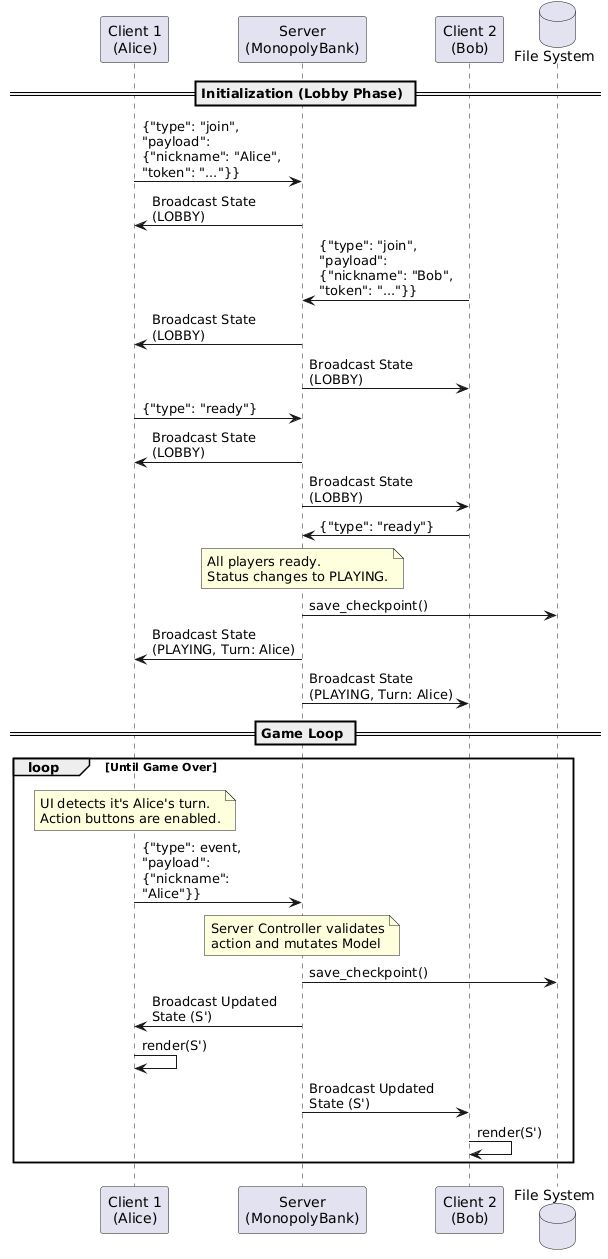
\includegraphics[width=\textwidth]{figures/sequence_diagram}
    \caption{Sequence diagram showing the Lobby initialization and the main Game Loop interaction.}
    \label{fig:sequence_diagram}
\end{figure}

\subsection{Behaviour}\label{behaviour}

The behavioral flow of the system revolves around the interaction between the Model, the View, and their dedicated Controllers.
Figure~\ref{fig:state_diagram} illustrates the complete lifecycle of a single user action, from the UI input to the global state broadcast.

\subsubsection*{Individual Component Behavior}
The components behave differently based on their responsibilities:
\begin{itemize}
    \item \textbf{\texttt{Monopoly} (Model) -- Stateful:} It is the core of the system.
    It maintains the current state of the game in memory.
    It mutates its internal variables only when invoked by the Server Controller.
    \item \textbf{\texttt{MonopolyView} (View) -- Stateful:} It holds the visual state of the board but knows nothing about the game logic.
    It runs an infinite loop waiting for user inputs.
    \item \textbf{\texttt{Controllers} -- Stateless:} Both the \texttt{ServerController} and \texttt{ClientController} act as pure functions or translators:
    the Client Controller maps player inputs into events, while the Server Controller maps events into Model method invocations.
    \item \textbf{\texttt{Serializer} -- Stateless:} It simply transforms objects into JSON strings and vice versa, without holding any memory of past transformations.
\end{itemize}

\subsubsection*{Updating the State of the System}
To guarantee strong consistency and prevent cheating, the system enforces a strict rule regarding state updates:
\begin{itemize}
    \item Only the \textbf{Server} (specifically the \texttt{Monopoly} Model,
    orchestrated by the \texttt{ServerController}) is in charge of updating the state of the game.
    \item The state is updated only when the Server receives a valid event message from a client (e.g., a \texttt{ROLL} or \texttt{BUY} event)
    or when a system timeout is triggered (e.g., a disconnected player is declared bankrupt).
    \item When a client terminal (\texttt{MonopolyUser}) captures an input, its controller generates an event dictionary.
    This event is serialized and sent to the server.
    The \texttt{ServerController} deserializes the event, manages the input, and asks the Model to check its correctness (e.g., checking if it is actually that player's turn).
    If valid, the Model computes the action and updates its internal variables.
    Finally, the Server Controller serializes the new state and sends it back to the clients,
    where the local controllers update their respective Views.
\end{itemize}

\begin{figure}[h]
    \centering
    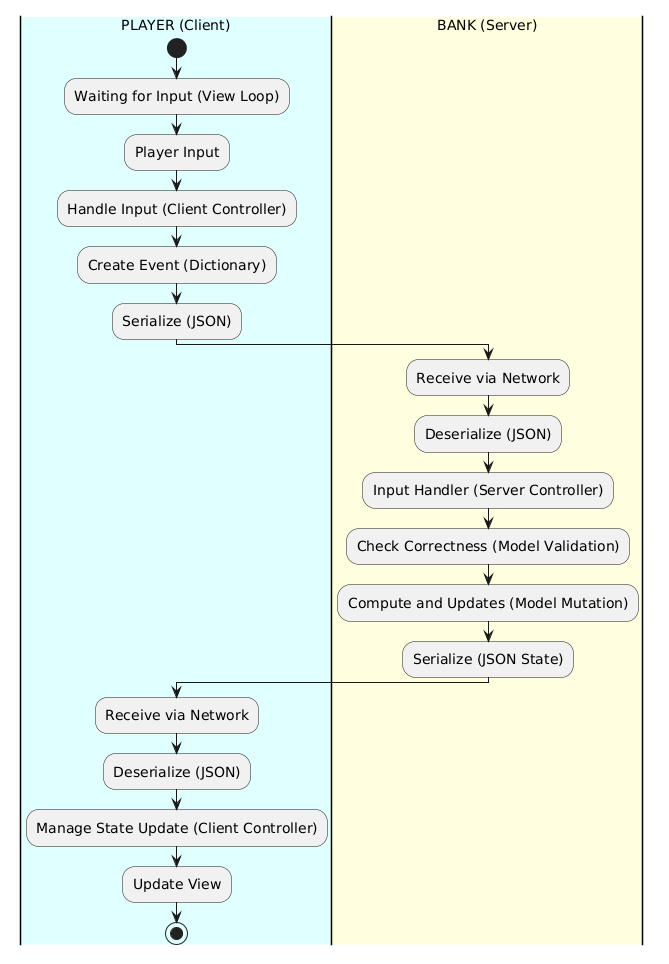
\includegraphics[width=\textwidth]{figures/state_diagram}
    \caption{Activity diagram based on the MVC pattern, showing the flow between the Player (Client) and the Bank (Server).}
    \label{fig:state_diagram}
\end{figure}

\subsection{Data and Consistency Issues}\label{data-and-consistency-issues}

The only data that needs to be stored are the checkpoint of the model,
that is the serialized JSON format of the actual state of the game including players token, and the players token.


The checkpoint is a file (\texttt{autosave.json}) where all the useful information needed to restore the game state in case of a server fail are saved.
It comprehends the serialized state of the game (players, balances, board ownerships, current turn)
along with the dictionary mapping player nicknames to their authentication tokens and the players token.
When the server starts it checks if a valid checkpoint is available and loads it.
During the game, on each event the server updates a checkpoint.


The players token are stored during the joining phase of a player (\texttt{nickname\_token.txt}).
It contains a unique UUID generated upon the first connection that is
used after a reconnection from a player by checking if the token provided by the user is the same of the token saved
on the server.


Both files are stored in the local filesystem, the checkpoint is stored on the server machine,
while the tokens file are stored on the clients machines.


There is no concurrency in reading and writing these data, each file is managed by the owner's machine clients or server.
There is a single copy of them, there isn't a backup, and they are not shared between nodes.
By relying on single local files without backups or distributed replication, the system achieves
\textbf{Strong Consistency} (there is a single source of truth).
The cost of this design is reduced \textit{Availability} and \textit{Fault Tolerance}: the files act as a Single Point of Failure.
If the server's disk fails or the file gets corrupted, the game cannot be restored.


Data must be consistent across the network to ensure the game works properly:
\begin{itemize}
    \item \textbf{Game State Sharing:} The server broadcasts the updated JSON state to all clients after every action so they can render the view synchronously.
    \item \textbf{Token Consistency:} The token provided by the client during a reconnection must strictly match the token saved in the server's checkpoint. If they are inconsistent, access is denied.
\end{itemize}


\subsection{Fault-Tolerance}\label{fault-tolerance}
The system is designed to handle the most common issues in multiplayer games: network drops, client disconnections, and unexpected server crashes.
\subsubsection{Data replication}
The only data replicated are the players token that are stored both on server and client, but it is needed only for
the authorization of a player to join a started game by checking if they are the same,
it cannot be used to restore a lost or corrupted data.
Tokens must be consistent in order to guarantee a right form of authentication during a client reconnection,
otherwise if one of the file is corrupted the authentication can fail and an allowed user cannot rejoin the game.

\subsubsection{Timeouts and Retry Mechanisms}\label{recovery}
The system implements timeout and retry loops to handle temporary network failures, preventing immediate game disruption:
\begin{itemize}
    \item \textbf{Server:} once the server lose connection a 90-second timeout starts.
    During this period of time if the connection is restored, the game restarts loading the last checkpoint saved.
    The game is set to \texttt{"CLOSED"} once the timeout ends.
    \item \textbf{Client:} once the client lose connection a 30-second timeout starts.
    During this period of time if the connection is restored, the game restarts.
    The player is set to \texttt{"bankruptcy"} once the timeout ends.
\end{itemize}


\subsubsection{Error handling}
The system uses TCP sockets for connections, so if a message fails to reach the peer, the exception is caught and the retry mechanisms starts.
If an error occurs during the joining phase the connection gets refused and a log is displayed on client's and server's CLI.
Errors that occurs in game are shown in the last event box on the GUI.

\subsection{Availability}\label{availability}

In the context of the CAP theorem, when a \textbf{network partition} occurs,
the system favors \textit{Consistency} over continuous \textit{Availability}, pausing the game to prevent desynchronization.
The behavior depends on which side of the network is isolated:
\begin{itemize}
    \item \textbf{Server isolation:} if the server lose the connection with the clients,
    each of them waits 90 seconds until considering the game closed.
    If the connection is reestablished, then the game restarts for all the client.
    \item \textbf{Client isolation:} if a client lose the connection with the server,
    the server stops the game for 30 seconds and waits to reestablish the connection.
    At the end of the 30 seconds the disconnected player is set as in bankruptcy and the game continues with the other alive players.
\end{itemize}

Having a single server that orchestrate the game and the connections yields to have a single point of failure.
This is handled by a set of recovery mechanism as the mechanism seen in section~\ref{fault-tolerance}.


\subsection{Security}\label{security}

The system implements a token-based authentication, introduced for handle players reconnections,
avoiding that a different user could take the place of a disconnected player only by using the same nickname.


During the joining phase of a client, a UUID token is created and stored in the local filesystem.
The token is then sent to the server along with his nickname.
After a disconnection, while reconnecting, the clients checks if there is a saved token and sends it with the nickname to the server.


The server stores a pair of token-nickname.
Once the disconnected player sends another JOIN message, the server checks if the token received is the same of the one stored during
the first JOIN.


There isn't a form of authorization because every user has the same access rights,
and a form of encryption, tokens and checkpoint are stored in clear.


\section{Implementation}\label{implementation}

This section details the technology-dependent choices adopted to implement the architectural design.

\subsubsection*{Network Protocols}
The system's communication is built on top of \textbf{TCP sockets}.
TCP provides a persistent, reliable, and ordered stream of data.
The server binds a dedicated socket for each connected client and maintains the connection open for the duration of the session.
This is ideal for a multiplayer board game where continuous state synchronization is required and packet loss (which could occur with UDP) must be avoided.

\subsubsection*{In-Transit Data Representation}
Messages exchanged between the server and clients are encoded in \textbf{JSON} format.
JSON was chosen because it's easy to parse and generate Python object.
A custom serializer and deserializer were implemented in order to parse the objects in a JSON format and reconstruct them from JSON to Python objects.

\subsubsection*{Database and Querying}
The system does not have a traditional relational (SQL) or NoSQL database.
Instead, it relies on the local filesystem.
The checkpoint is saved directly as a JSON file (\texttt{autosave.json}).
Consequently, there is no formal query language involved,
the system performs direct I/O reads and writes to dump or load the entire game state and players token.

\subsubsection*{Authentication}
The system implements a lightweight custom \textbf{Token-based Authentication} for session recovery.
Upon the first connection, a standard UUID is generated.
This token is saved in clear text on the client's machine and mapped alongside the checkpoint dictionary on the server.
Reconnecting clients must provide this exact UUID to prove their identity and reclaim their seat.

\subsubsection*{Authorization}
All users have the exact same role (``Player'').
The only type of authorization implemented in the system is made using the nicknames that
the server uses to checks in the internal game state before authorizing any state-mutating command,
ensuring that players can only interact when it is legally their turn.

\subsection{Technological details}\label{technological-details}

The system is entirely developed in Python 3.
The framework used for the client's View is PyGame that provides the rendering engine for drawing the board, managing the game loop,
and capturing hardware events (such as mouse clicks for the action buttons).


\section{Validation}\label{validation}

\subsection{Automatic Testing}\label{automatic-testing}

The core of the model has been tested automatically, along with serialization and deserialization.

Individual components that do not rely on active network sockets or GUI rendering were unit-tested using the \textbf{\texttt{pytest}} framework.
The primary targets were:
\begin{itemize}
    \item \textbf{Model}: main entities were tested on different scenarios for every game phase (\texttt{LOBBY}, \texttt{PLAYING}, \texttt{CLOSED}, \texttt{PAUSED}),
                            with different number of players, and on player disconnection and reconnection.
    \item \textbf{Data Serialization:} \texttt{Serializer} and \texttt{Deserializer} were tested on each entity,
                                        on the full game state and on unsupported data.
\end{itemize}

\subsection{Acceptance test}\label{acceptance-test}
To validate the overall user experience, the system has been tested through an extensive manual acceptance testing.

The system has been tested on the communication, interaction, and integration among all components across a Local Area Network (LAN).
The setup involved deploying the \texttt{MonopolyBank} server on one physical machine and connecting multiple \texttt{MonopolyUser} clients from different or same hosts.
The standard game loop (joining, rolling, buying, ending turns) was tested focusing also on corner cases and fault-tolerance mechanisms:
  \begin{itemize}
      \item \textit{Network Partitions:} Unexpected client disconnections (e.g., physically disabling a machine's Wi-Fi adapter) were simulated
                    to verify the 30-second timeout and the subsequent bankruptcy logic.
      \item \textit{Crash Recovery:} Server process were forcefully killed to ensure the \texttt{autosave.json} checkpoint
                    was correctly generated and capable of restoring the paused game state upon server reboot.
      \item \textit{Security Authentication:} Reconnections were tested verifying that dropped players could successfully
                    rejoin using their local UUID tokens, and that unauthorized connections were correctly rejected.
  \end{itemize}

These tests have been done manually because the client is tightly coupled with \texttt{PyGame}.
Verifying that UI elements (tokens, action buttons, properties) are rendered at the correct coordinates
and respond to hardware mouse events is particularly complex.
Furthermore, simulating TCP connections, physical network drops, socket timeouts across multiple nodes would have added
more complexity if tested automatically.

\section{Deployment}\label{deployment}

To prepare the environment to run the system locally,
there are three main steps: cloning the repository, setting up the server (via Docker or locally), and starting the client terminals.

\subsubsection*{Prerequisites and Software Versions}
To run the project, the following software must be installed on the host machines:
\begin{itemize}
    \item \textbf{Python:} Version \texttt{3.10} or higher.
    \item \textbf{Dependencies:} The project requires two external libraries,
    specified in the \texttt{requirements.txt} file: \texttt{pygame>=2.0.0} (for the client GUI)
    and \texttt{psutil>=5.0.0} (for server network utilities).
    \item \textbf{Docker \& Docker Compose} (Optional for the server deployment).
\end{itemize}

\subsubsection*{Containerization (Server)}
The \texttt{MonopolyBank} server is fully containerized.
\begin{itemize}
    \item \textbf{Dockerfile:} It starts from a lightweight \texttt{python:3.10-slim} image.
    It copies the \texttt{requirements.txt} first to leverage Docker's layer caching during the \texttt{pip install} phase.
    \item \textbf{Docker Compose:} The \texttt{docker-compose.yml} maps the container's exposed port to the host's port (\texttt{8080:8080}).
    It maps a local volume (\texttt{./checkpointing:/app/checkpointing}).
    This choice ensures that the \texttt{autosave.json} checkpoint file persists on the host machine even if the container
    is stopped or destroyed, guaranteeing fault tolerance.
\end{itemize}

\subsubsection*{Step-by-Step Installation and Startup Instructions}\label{installation}

\begin{enumerate}
    \item \textbf{Clone the Repository:}
    Open a terminal and clone the project source code.
    \begin{verbatim}
    git clone https://github.com/22Daniele/DS-monopoly-clone
    cd dmonopoly
    \end{verbatim}

    \item \textbf{Start the Server:}
    You can run the server using Docker Compose:
    \begin{verbatim}
    docker-compose up --build
    \end{verbatim}
    \textit{Expected Outcome:} Docker will build the image and the server will begin listening on port 8080.
    \\
    Alternatively, to run it locally without Docker:
    \begin{verbatim}
    pip install -r requirements.txt
    python serverMain.py
    \end{verbatim}

    \item \textbf{Start the Clients:}
    On the players' machines, ensure Python is installed, then install the requirements and launch the client script.
    \begin{verbatim}
    pip install -r requirements.txt
    python clientMain.py <SERVER_IP> <PORT> <NICKNAME>
    \end{verbatim}
    \textit{Expected Outcome:} A PyGame graphical window will open, presenting the initial Lobby screen.
    The CLI will log the successful connection to the server or display a rejection message if the lobby is full.
\end{enumerate}
\vspace{0.5cm}
\noindent\textbf{Important Note on Docker:} \\
If the server is deployed using Docker, the IP address automatically detected and printed in the server's console logs is the
Docker's internal virtual network rather than the host machine's actual IP.
When connecting clients from different physical machines, users must ignore the internal Docker IP and instead provide
the host machine's real IP address as the connection endpoint.


\subsubsection*{Environment Variables and Configuration}
No external \texttt{.env} files or configuration files are required.
The server automatically creates the \texttt{checkpointing} directory,
and the clients automatically generate the \texttt{tokens} directory upon their first launch.
Network configurations (like dynamic IP resolution) are handled internally by the code via the \texttt{psutil} library.

\section{User Guide}\label{user-guide}
This section is a guide on how to interact with the Monopoly system once the deployment steps
(described in Section~\ref{deployment}) have been completed.

\subsubsection{LOBBY phase}
During this phase, clients (up to 4) can join the game and press the ready button shown on the GUI.
Once all the player in the lobby (at least 2) are ready, the game enters in the next phase.
\begin{figure}[h]
    \centering
    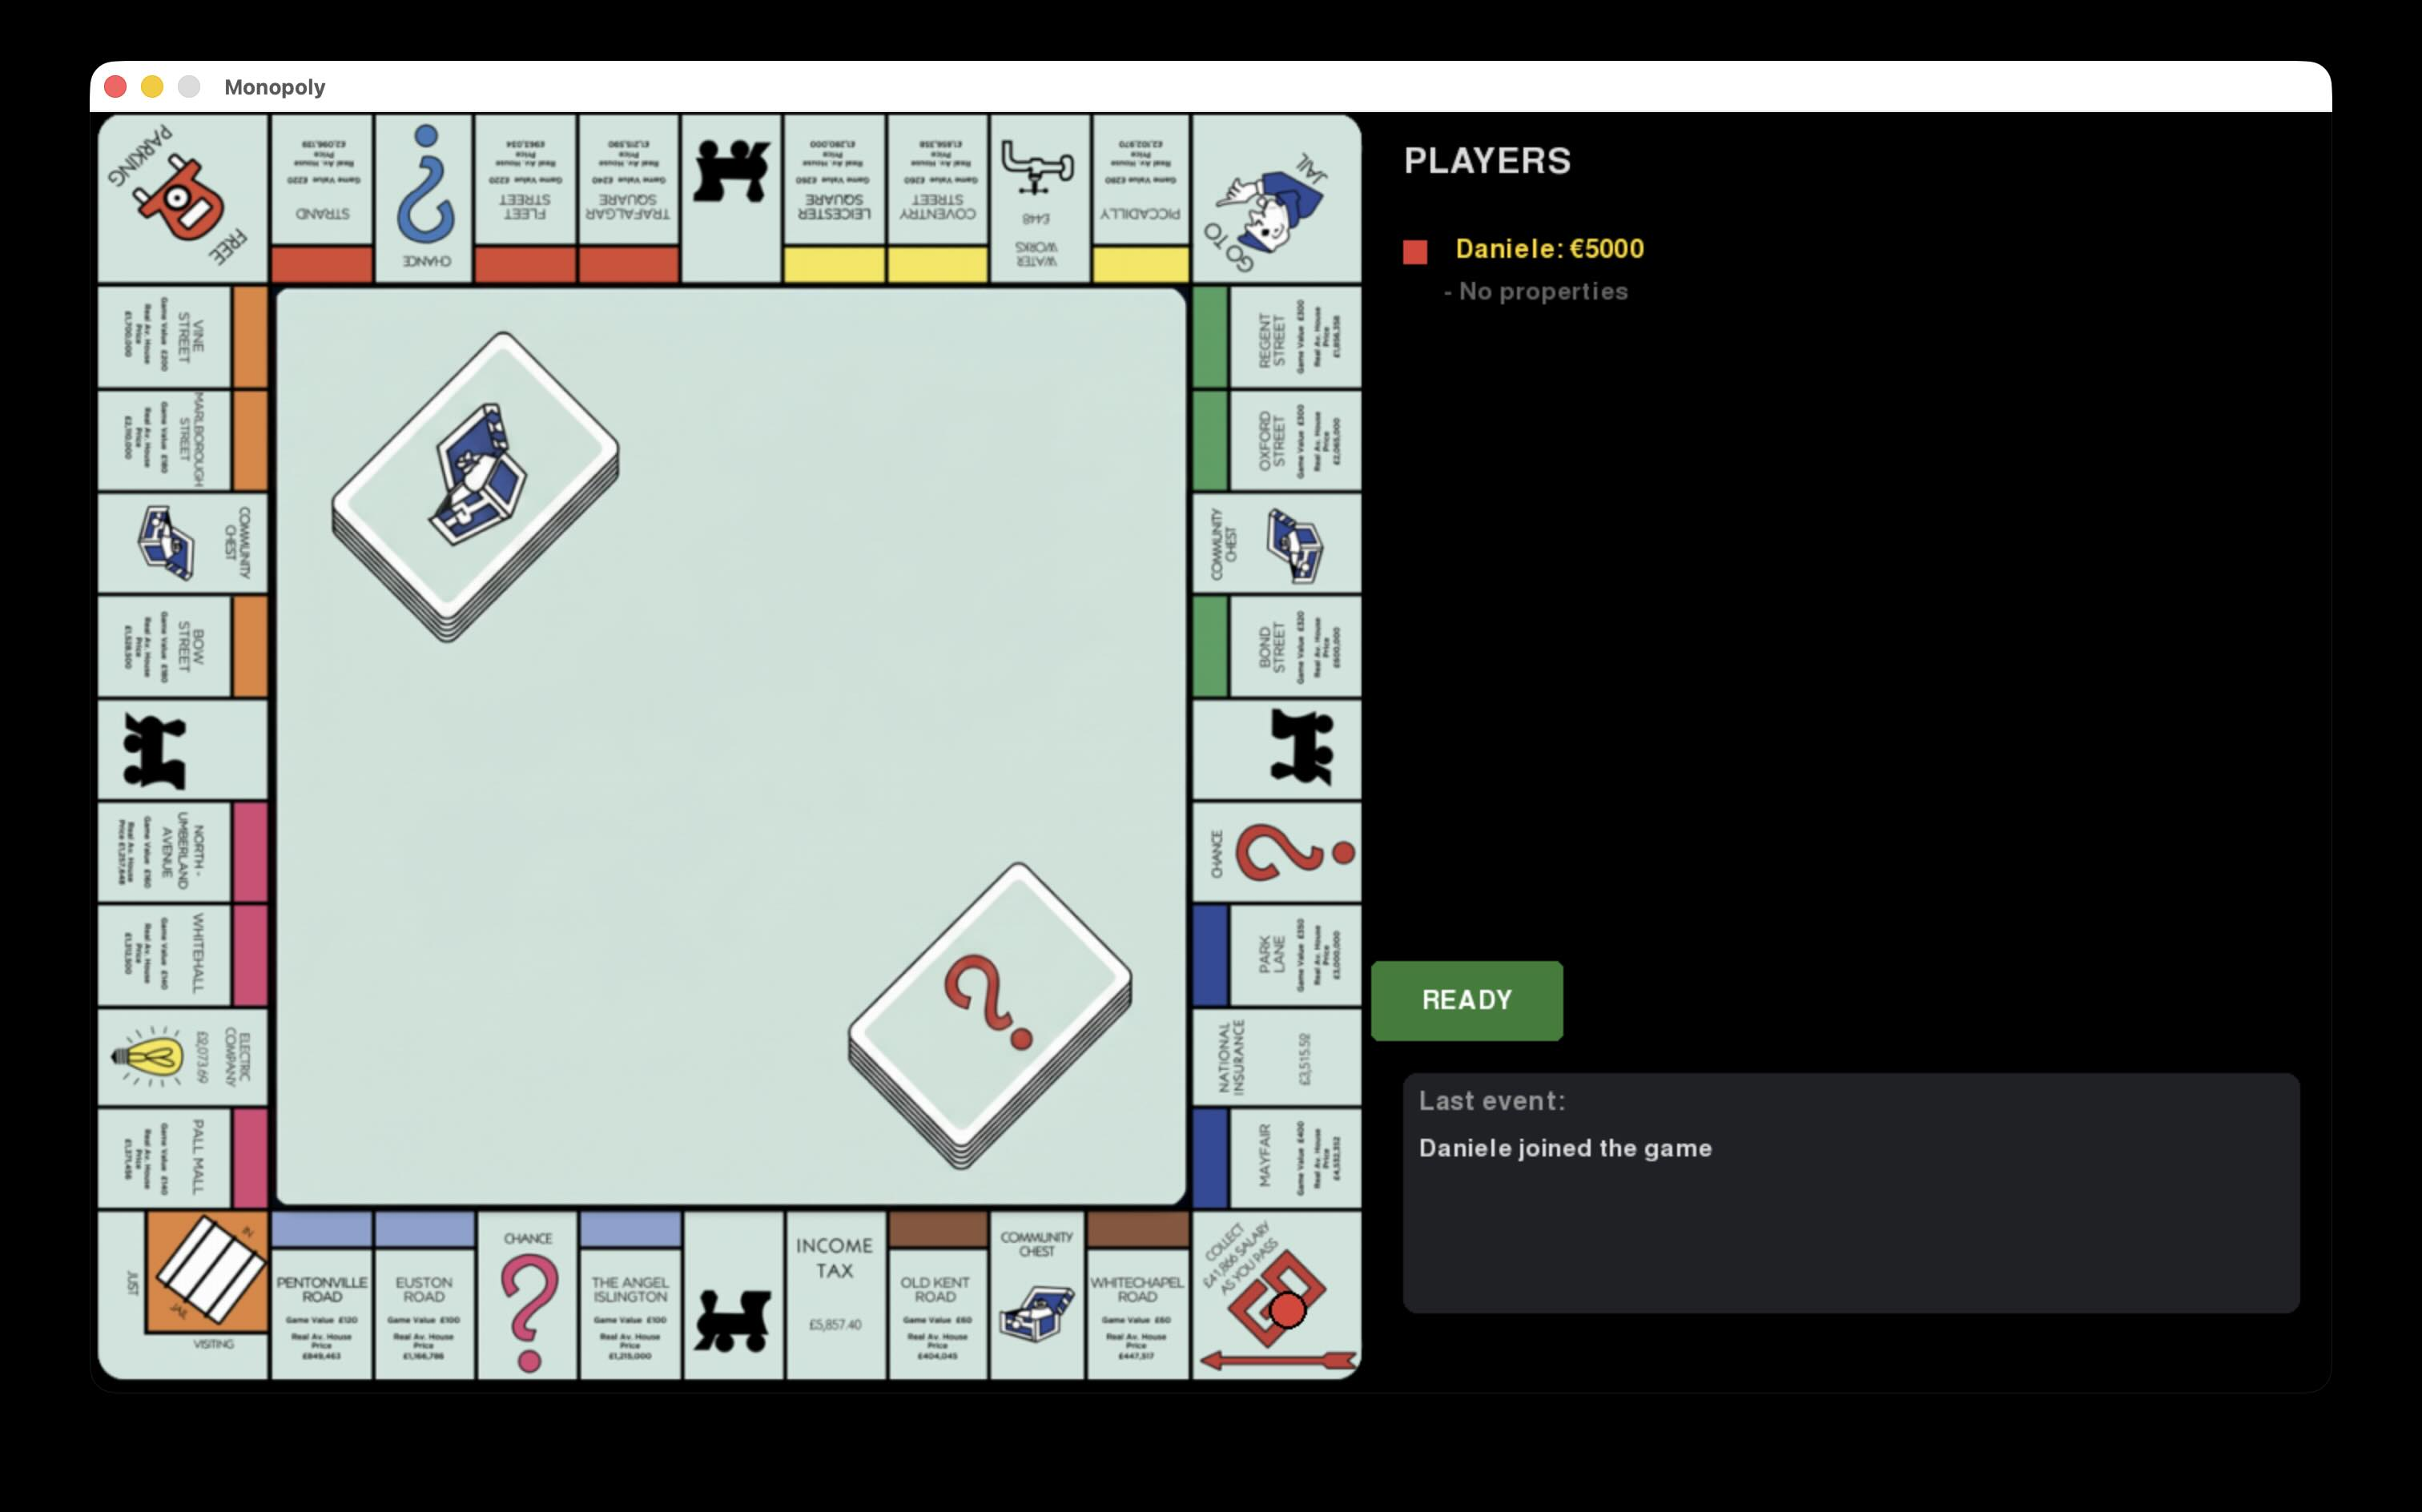
\includegraphics[width=0.7\textwidth]{figures/lobby}
    \caption{The client GUI during the LOBBY phase.}
    \label{fig:gui_lobby}
\end{figure}

\subsubsection{PLAYING phase}
In this phase the monopoly match starts, every player is initialized with a balance of 5000 coins and 5 random properties.
Players should see the board on the left of the window and a dashboard showing players information and last event log on the right.
Each player in turn can see and press on their screen buttons to perform actions
\begin{itemize}
    \item \textbf{Your Turn:} When it is your turn, the GUI dynamically enables action buttons (e.g., \texttt{ROLL}, \texttt{BUY}, \texttt{BUILD}, \texttt{END\_TURN}).
    Click these buttons to perform your allowed moves.
    The action is processed by the server, and the game information on the GUI updates for everyone.
    \item \textbf{Others' Turn:} When it is not your turn, no actions are allowed.
    The action buttons are hidden or disabled.
    You act as a spectator, watching the real-time updates triggered by the active player.
\end{itemize}

\begin{figure}[h]
    \centering
    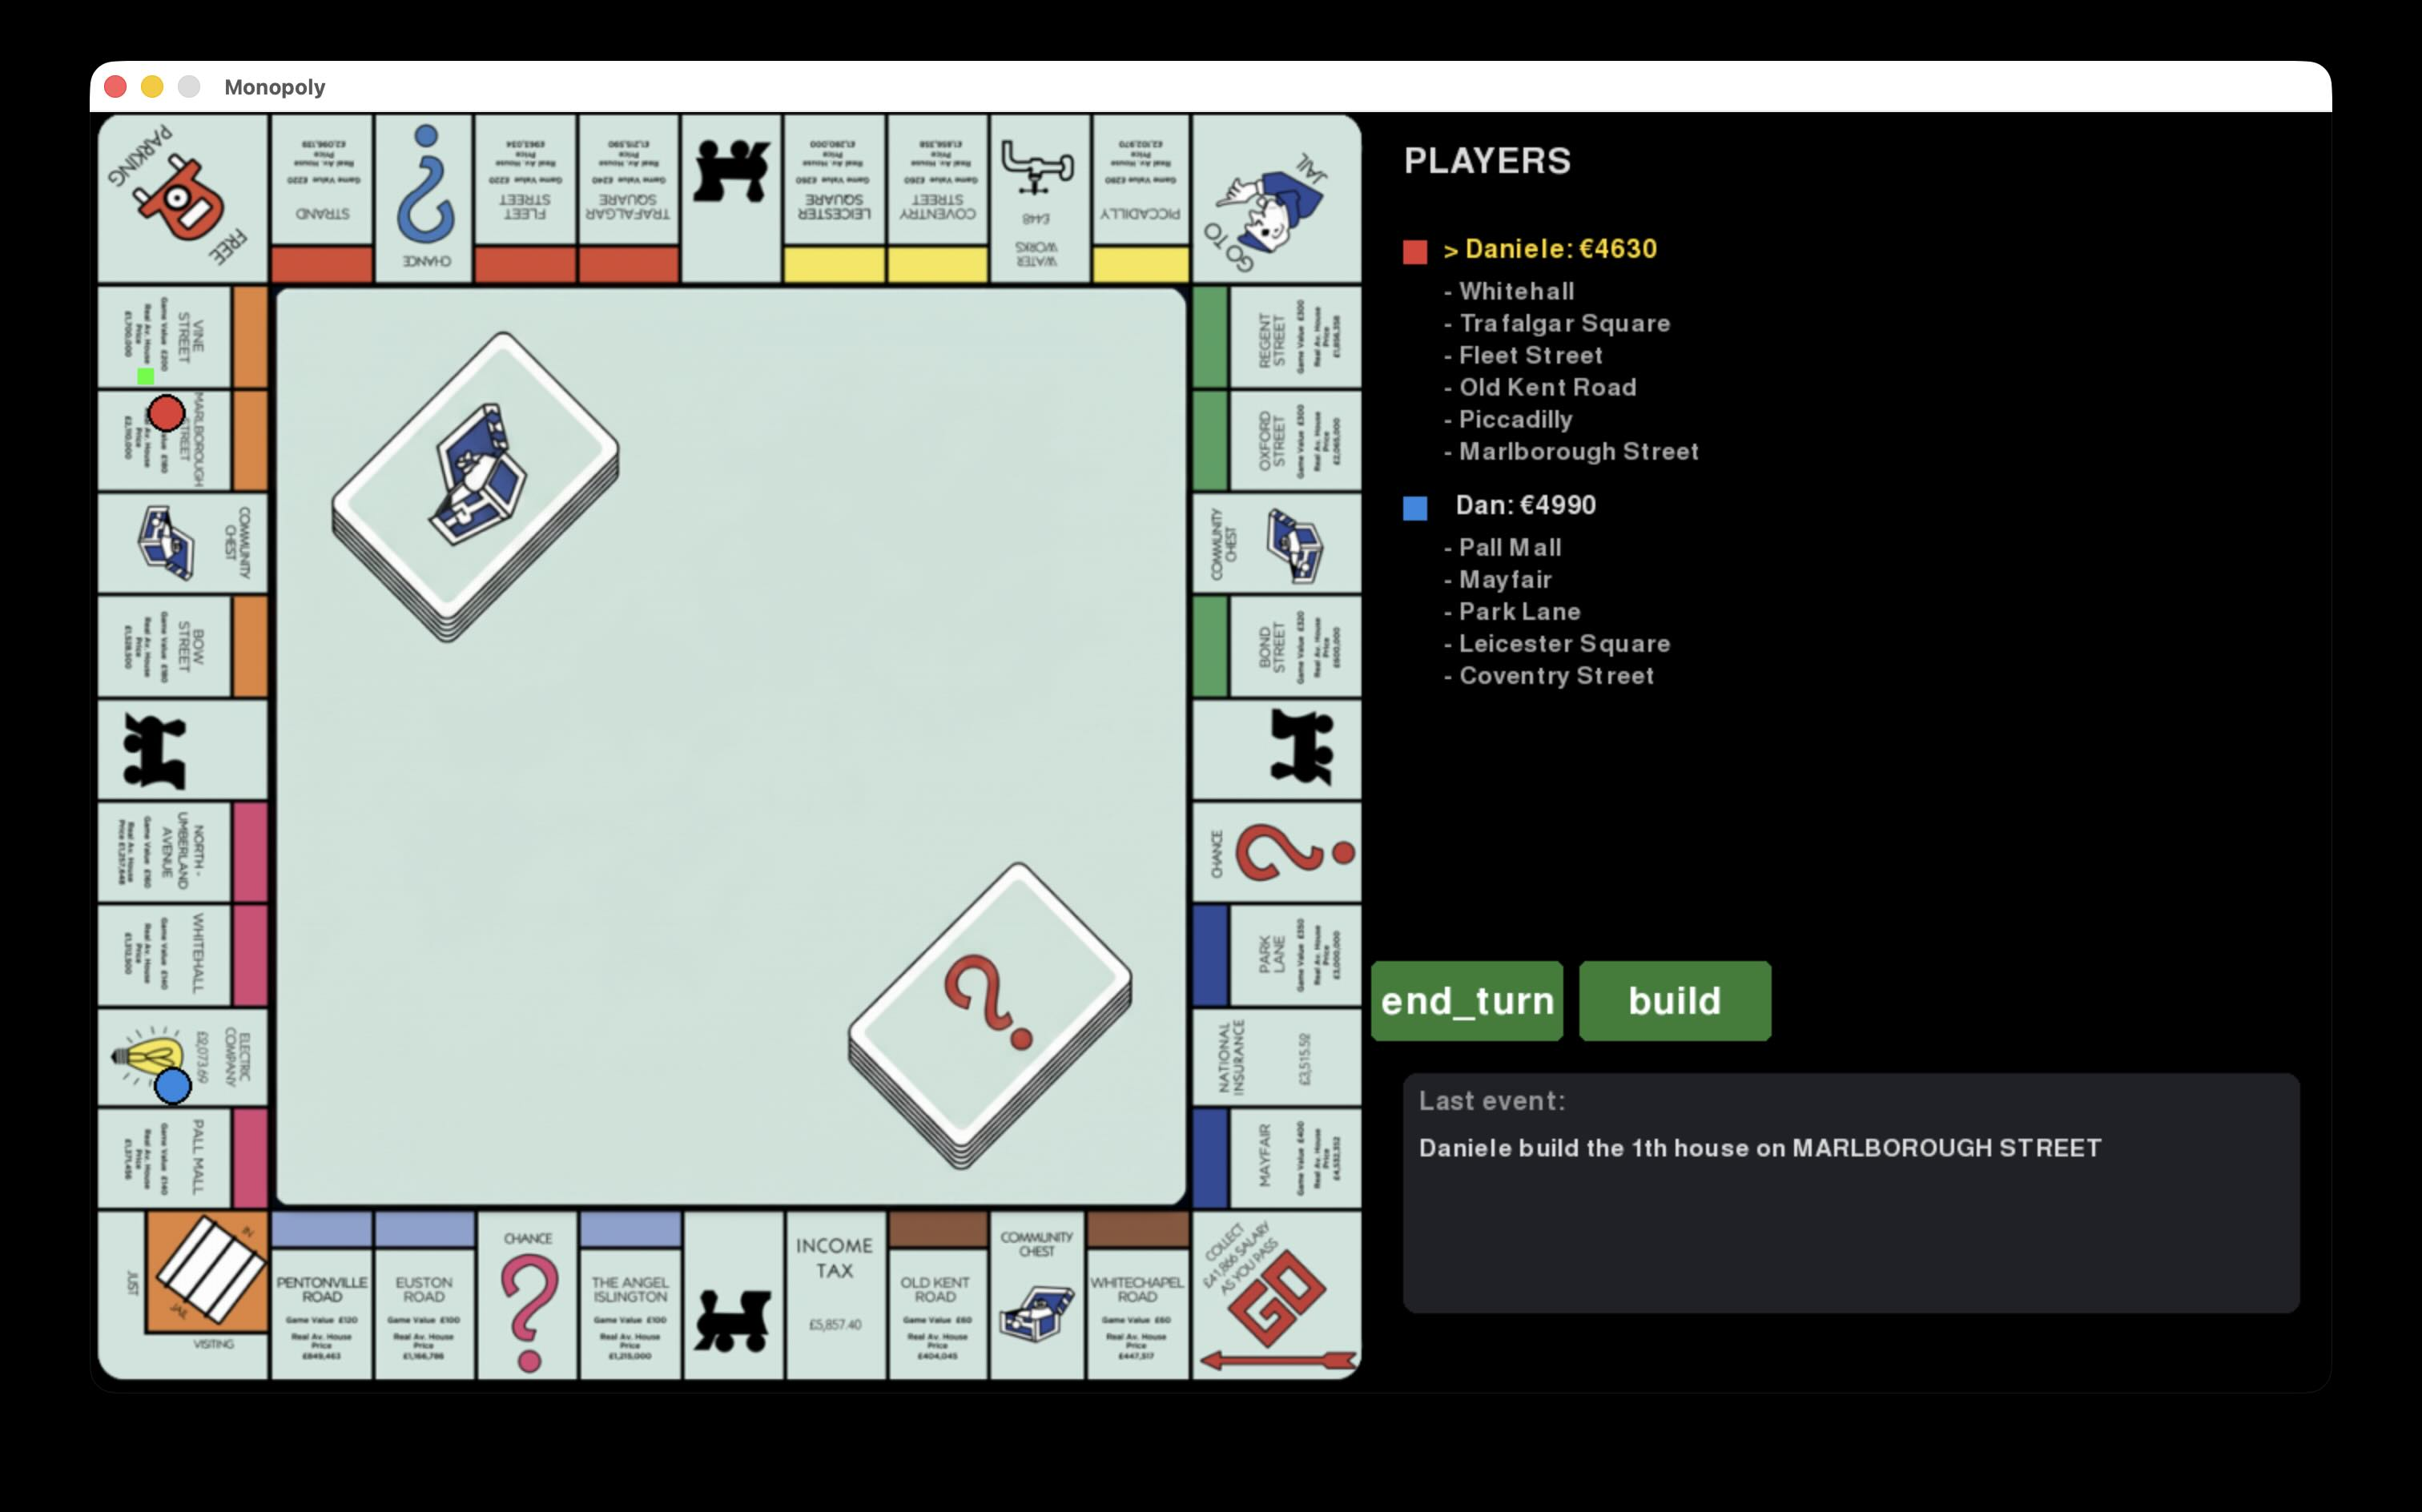
\includegraphics[width=\textwidth]{figures/playing}
    \caption{The game interface during the PLAYING phase.}
    \label{fig:gui_playing}
\end{figure}

\subsubsection{PAUSED phase}
If a client loses the connection mid-game, the system enters the PAUESED phase,
stopping immediately the game and starting the recovery mechanism~\ref{recovery}.
During this phase all the players can do nothing.

\begin{figure}[h]
    \centering
    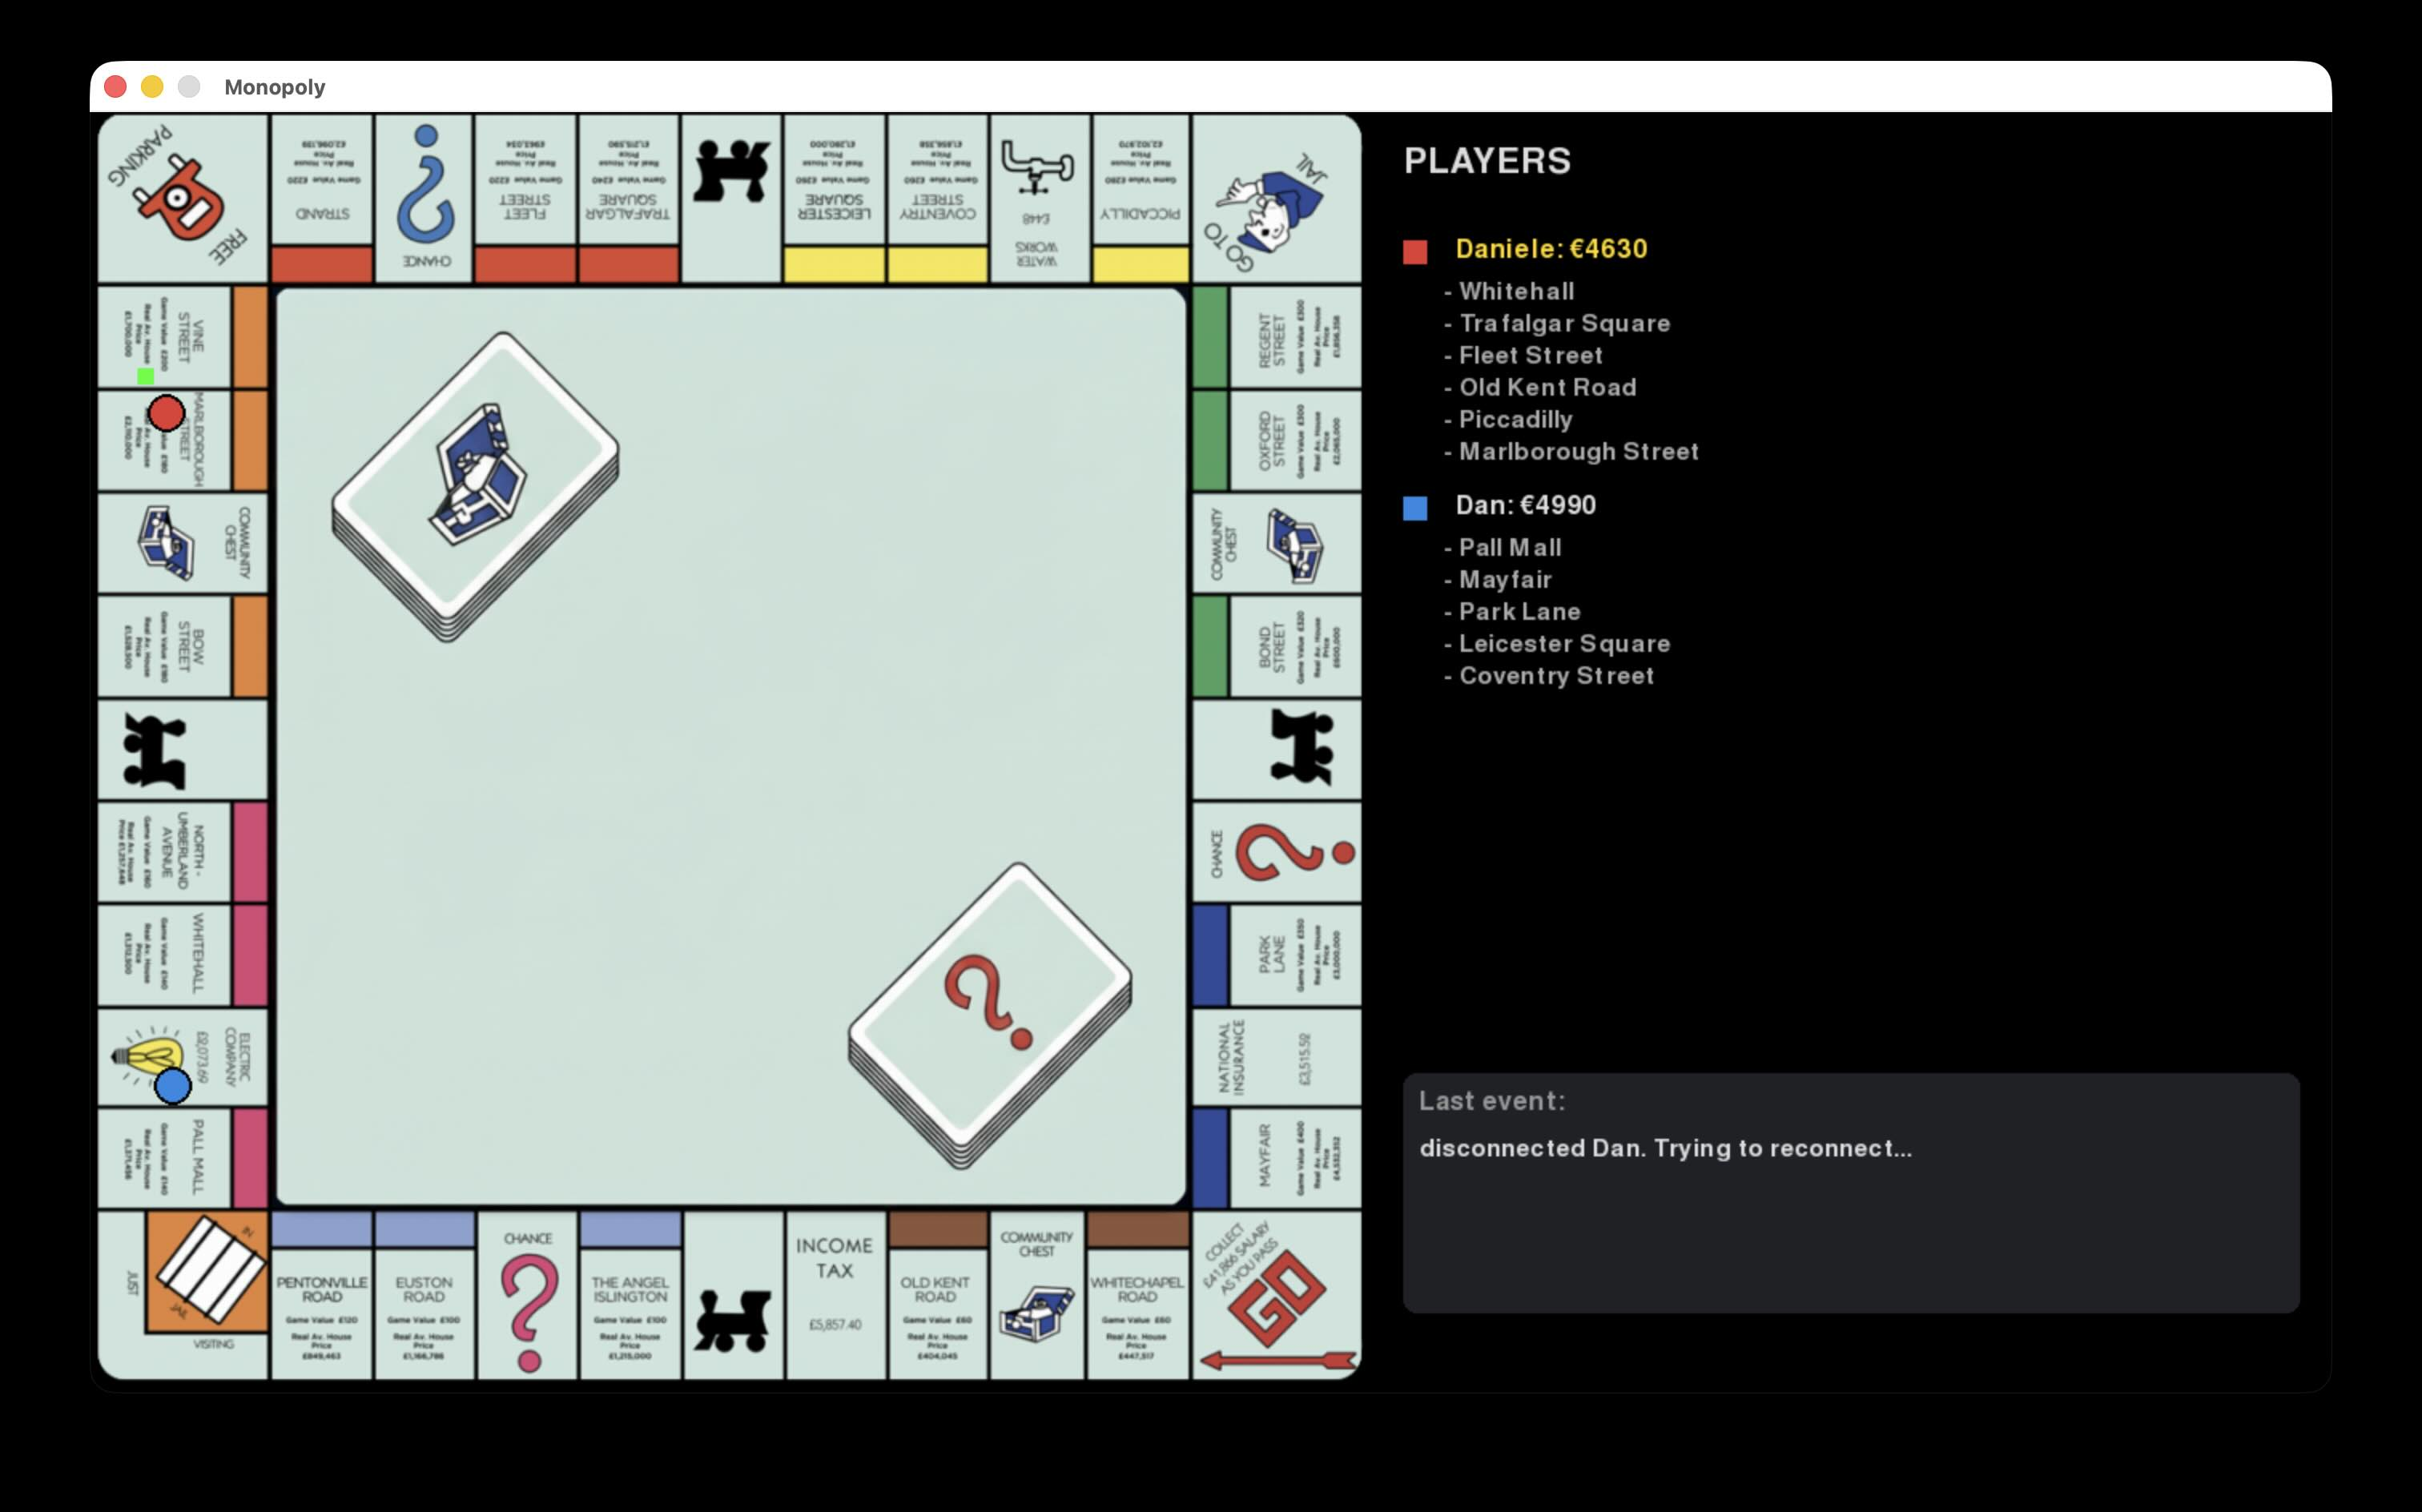
\includegraphics[width=\textwidth]{figures/paused}
    \caption{The game interface during the PAUSED phase.}
    \label{fig:gui_paused}
\end{figure}

\subsubsection{CLOSED phase}
The game ends when only one active player is left (i.e., everyone else is bankrupt or has permanently disconnected) and enters in the CLOSED phase.
The winner is implicitly declared, and no further actions can be performed by the users.

\begin{figure}[h]
    \centering
    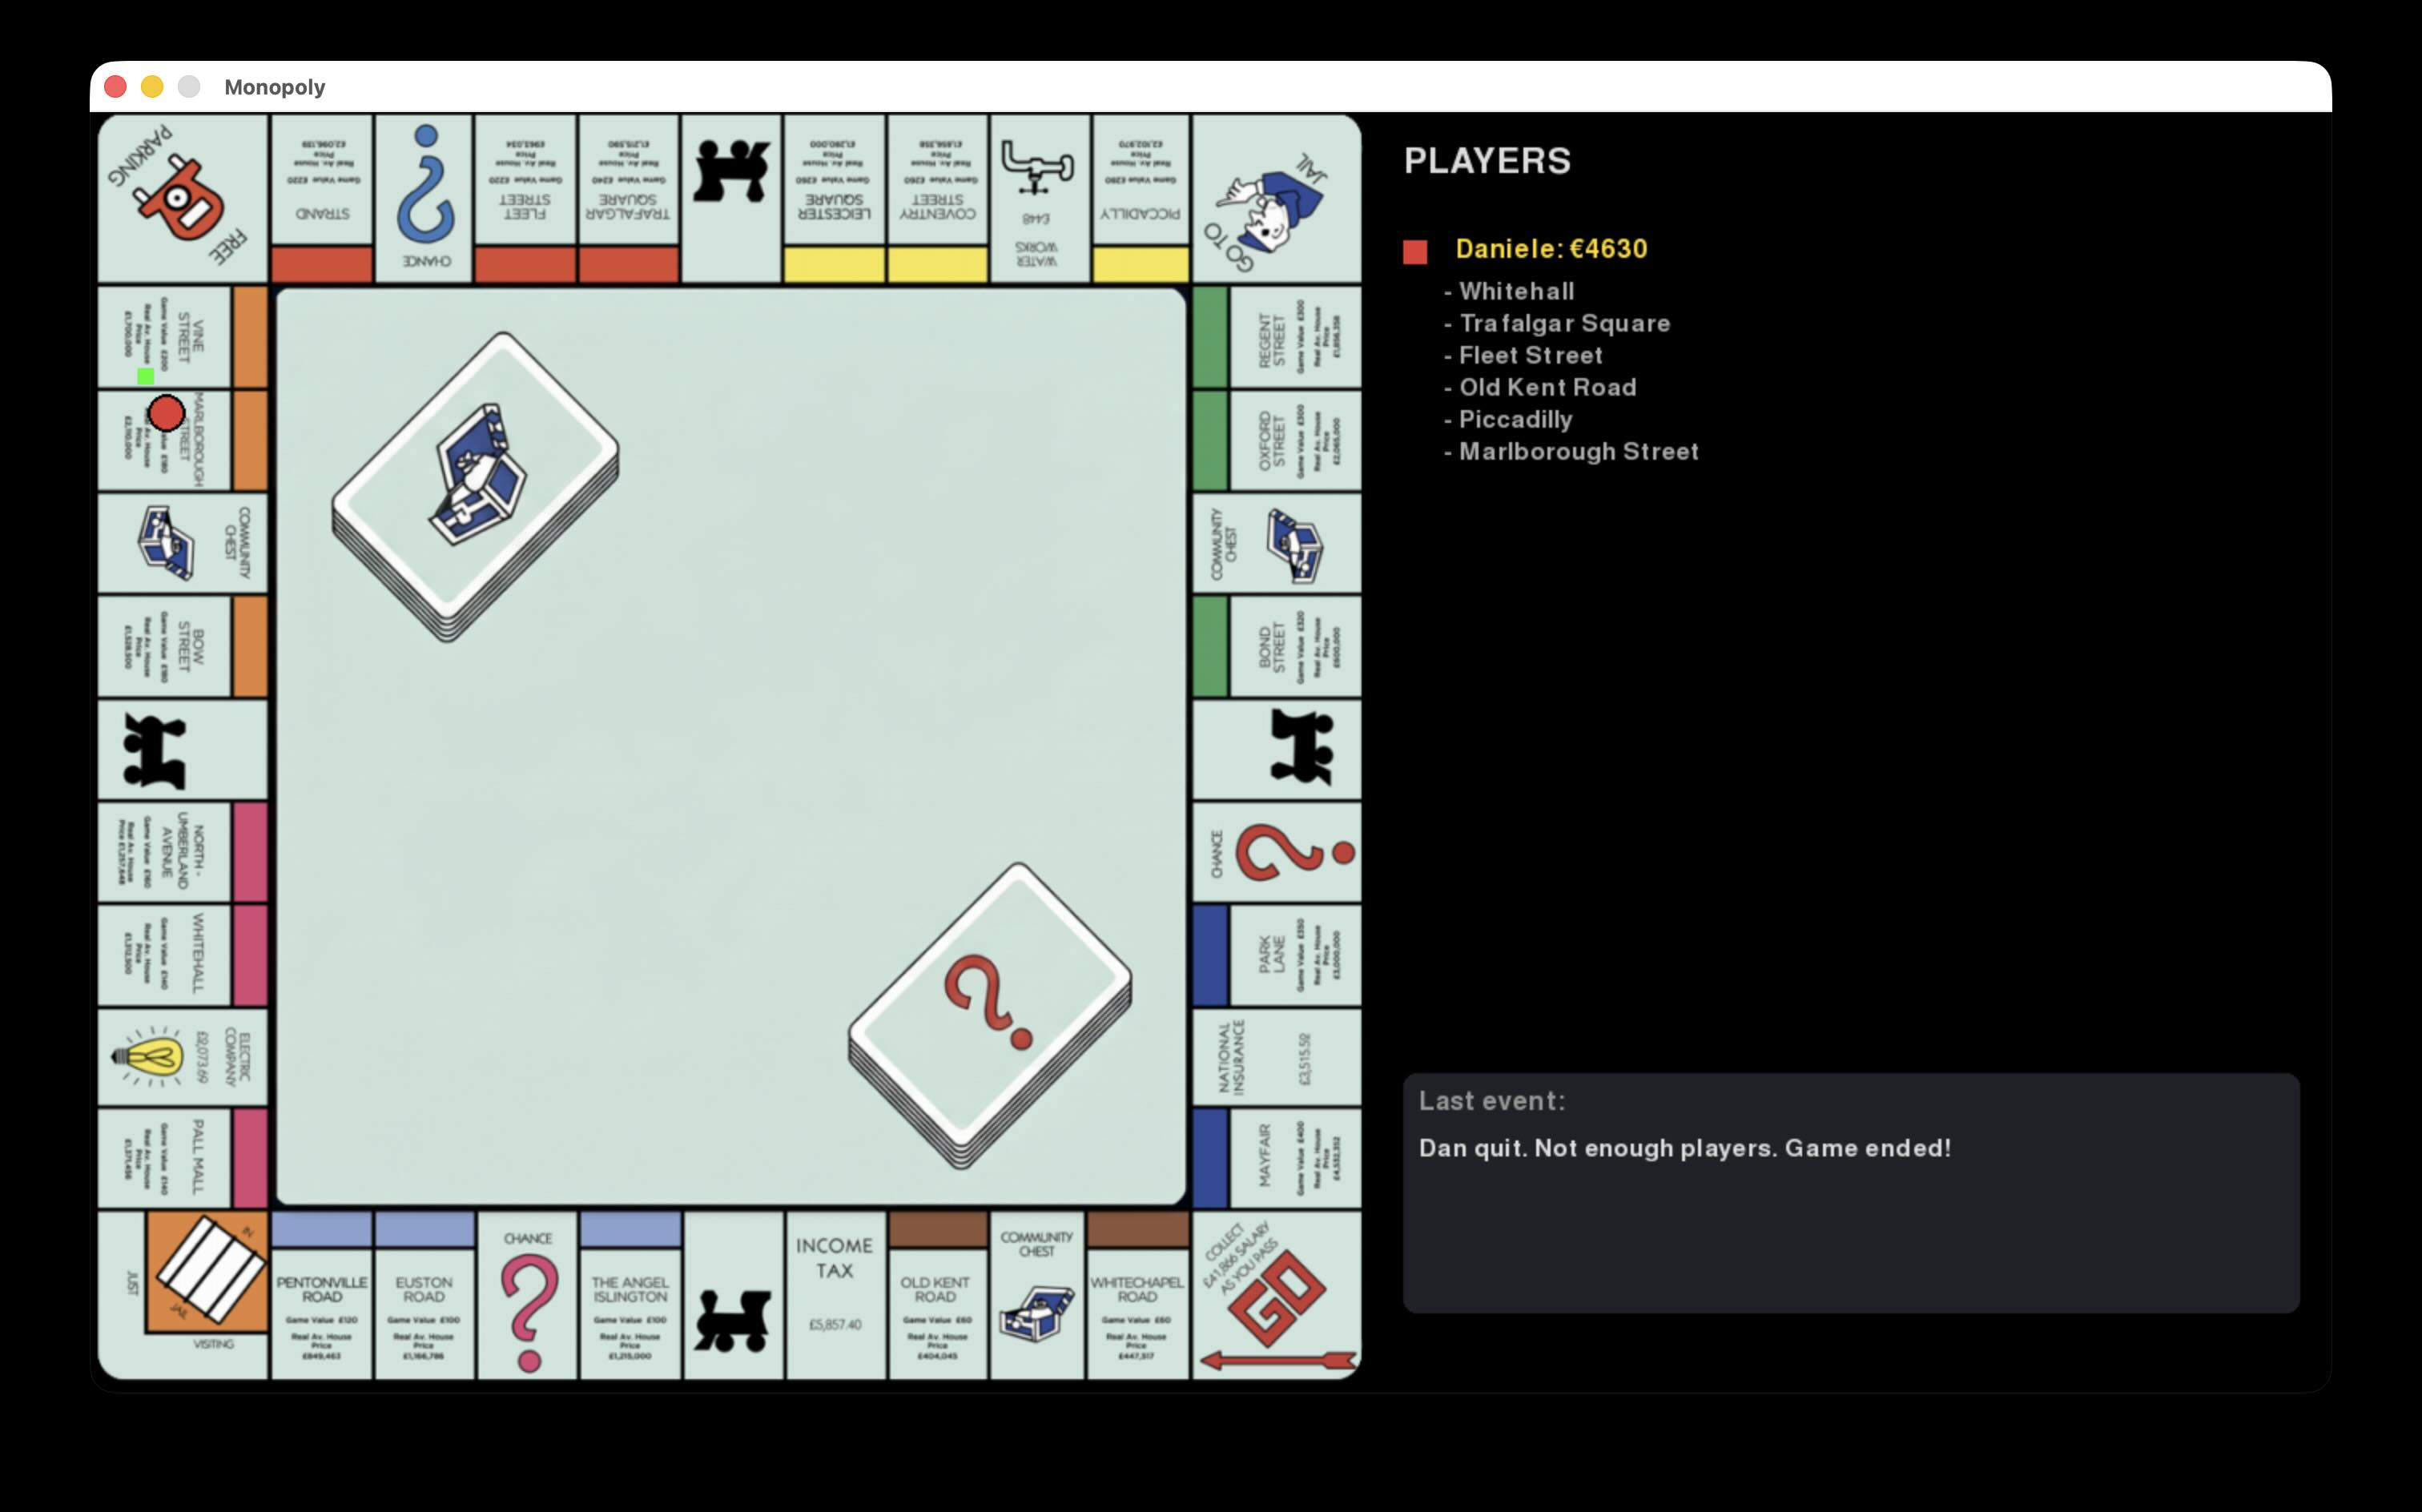
\includegraphics[width=\textwidth]{figures/closed}
    \caption{The game interface during the CLOSED phase.}
    \label{fig:gui_closed}
\end{figure}

\subsubsection{Shutting Down the System}
\begin{itemize}
    \item \textbf{Clients:} Users can gracefully leave the game at any time simply by closing the PyGame window.
    \item \textbf{Server:} Once all clients have disconnected and the game is empty, the Python server process shuts down automatically.
    However, if the server was started via \texttt{docker-compose}, the Docker daemon will automatically restart it,
    immediately readying the system to host a new game session.
\end{itemize}

\begin{itemize}
  \item how to use your software?
  %
  \begin{itemize}
    \item provide instructions
    \item provide expected outcomes
    \item provide screenshots if possible
  \end{itemize}
\end{itemize}

\section{Self-evaluation}\label{self-evaluation}

\begin{itemize}
  \item An individual section is required for each member of the group
  \item Each member must self-evaluate their work, listing the strengths and weaknesses of the product
  \item Each member must describe their role within the group as objectively as possible.
\end{itemize}

It should be noted that each student is only responsible for their own section.

\section{Future works}\label{future-works}

Discuss possible future works, improvements, extensions, optimizations, etc.

Also discuss here any unimplemented feature, and how you would have implemented it.

\bibliographystyle{plain}
\bibliography{references}

\end{document}
